\documentclass[../../deep_learning_notes.tex]{subfiles}
\begin{document}
%%%%%%%%%%%%%%%%%%%%%%%%%%%%%%
\section{Recurrent Neural Network (RNN)}
The building block of any recurrent network, RNN has the following form of the forward pass through the network
\begin{align*}
    h_{0} &= \bm{0}_{h}\\
    h_{t} &= f_{h}(x_{t}W_{xh} + h_{t-1}W_{hh} + b_{h}) \quad \forall t = 1, 2, \ldots, T\\
    y_{t} &= f_{y}(h_{t}W_{yh} + b_{y})
\end{align*}

which is demonstrated diagramatically in figure \ref{fig:rnn_1}. Based in the dimensions of the input and hidden state, we can calculate the sizes of the weight matrices. $W_{x}$ is the same size as input size $\times$ hidden state size, $W_{h} \in \mathcal{R}^{4\times 3}$. $W_{h}$ will be a square matrix since it converts previous hidden state to and output of same size as hidden state. $W_{h} \in \mathcal{R}^{3 \times 3}$. The output is a single transformation from size $3$ to $1$, $W_{y} \in \mathcal{R}^{3 \times 1}$. There will be one bias vector for the hidden layer and one for the output. Activations are most of the time element wise transformations and maintain the size (if not the shape) of output. \newline
Thus, the total parameters in this network are
\begin{align*}
    ((4\times 3) + (3 \times 3 + 3)) + (3 \times 1 + 1) = 28
\end{align*}

\begin{figure}[h]
    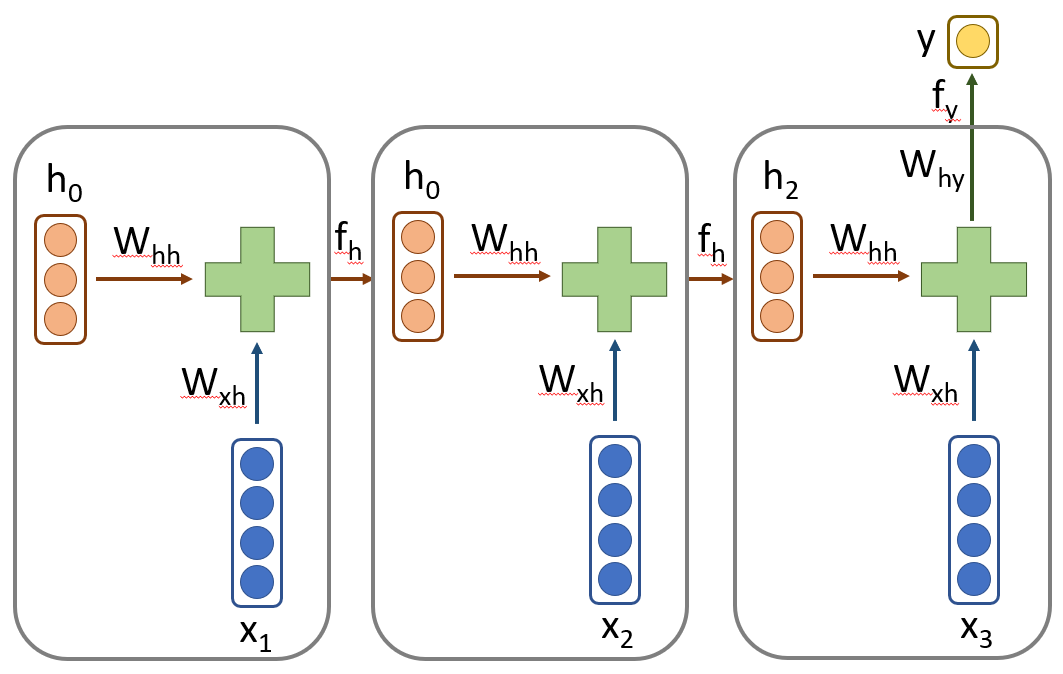
\includegraphics[scale=0.6]{rnn_1}
    \centering
    \caption {Diagramatic representation of an RNN. This particular model has $3$ timesteps, input vector has dimension of $4$ and hidden state has dimension of $3$. The output is a single number and this is a many to one type of architecture.}
    \label{fig:rnn_1} %\ref{fig:rnn_1}
\end{figure}

The main advantage of this approach is reduced number of parameters. Suppose, we used a dense neural network for doing a similar task. Then the input layer will be of size number of timesteps $\times$ input size which is $12$. Hidden layer will be of size $9$ and the output of size $1$. Total parameters will be
\begin{align*}
    (12 \times 9 + 9) + (9 \times 1 + 1) = 127
\end{align*}
which is at least $4$ times more parameters. Clearly we benefit by using the shared weight structure of RNN. However, in more advanced architectures, we may have more complicated structures using gates which can increase the parameters.\newline

Often, we will encounter a different mathematical notation for RNN that uses a single weights matrix to calculate the hidden state
\begin{align*}
    h_{0} &= \bm{0}_{h}\\
    h_{t} &= f_{h}([h_{t-1}, x_{t}]W_{h} + b_{h}) \quad \forall t = 1, 2, \ldots, T\\
    y &= f_{y}(W_{yh}h_{T} + b_{y})
\end{align*}
where everything else except the hidden state calculations remains the same. The notation $[h_{t-1}, x_{t}]$ denotes horizontal stacking of these two vectors (note that the horizontal axis is the variables dimension). Similarly, the new weights matrix $W_{h}$ is the vertical concatenation of the previous $W_{hh}$ and $W_{xh}$. This allows for faster implementation since we will not two separate matrix multiplications to calculate the hidden state.
\end{document}